
\begin{section}{Experimentación}
 No se comparó la simulación contra un fluido real bajo las mismas condiciones. Sin embargo la simulación parece reflejar correctamente el comportamiento de un fluido, como puede apreciarse en el \href{https://www.youtube.com/watch?v=D8JOELu8uAs}{mapa de velocidad total codificado por color}, o en el \href{https://www.youtube.com/watch?v=_JisfmOIEdU}{campo vectorial} de las figuras \ref{fig:sim_hm_all} y \ref{fig:sim_vf_all}
~\\
\begin{figure*}
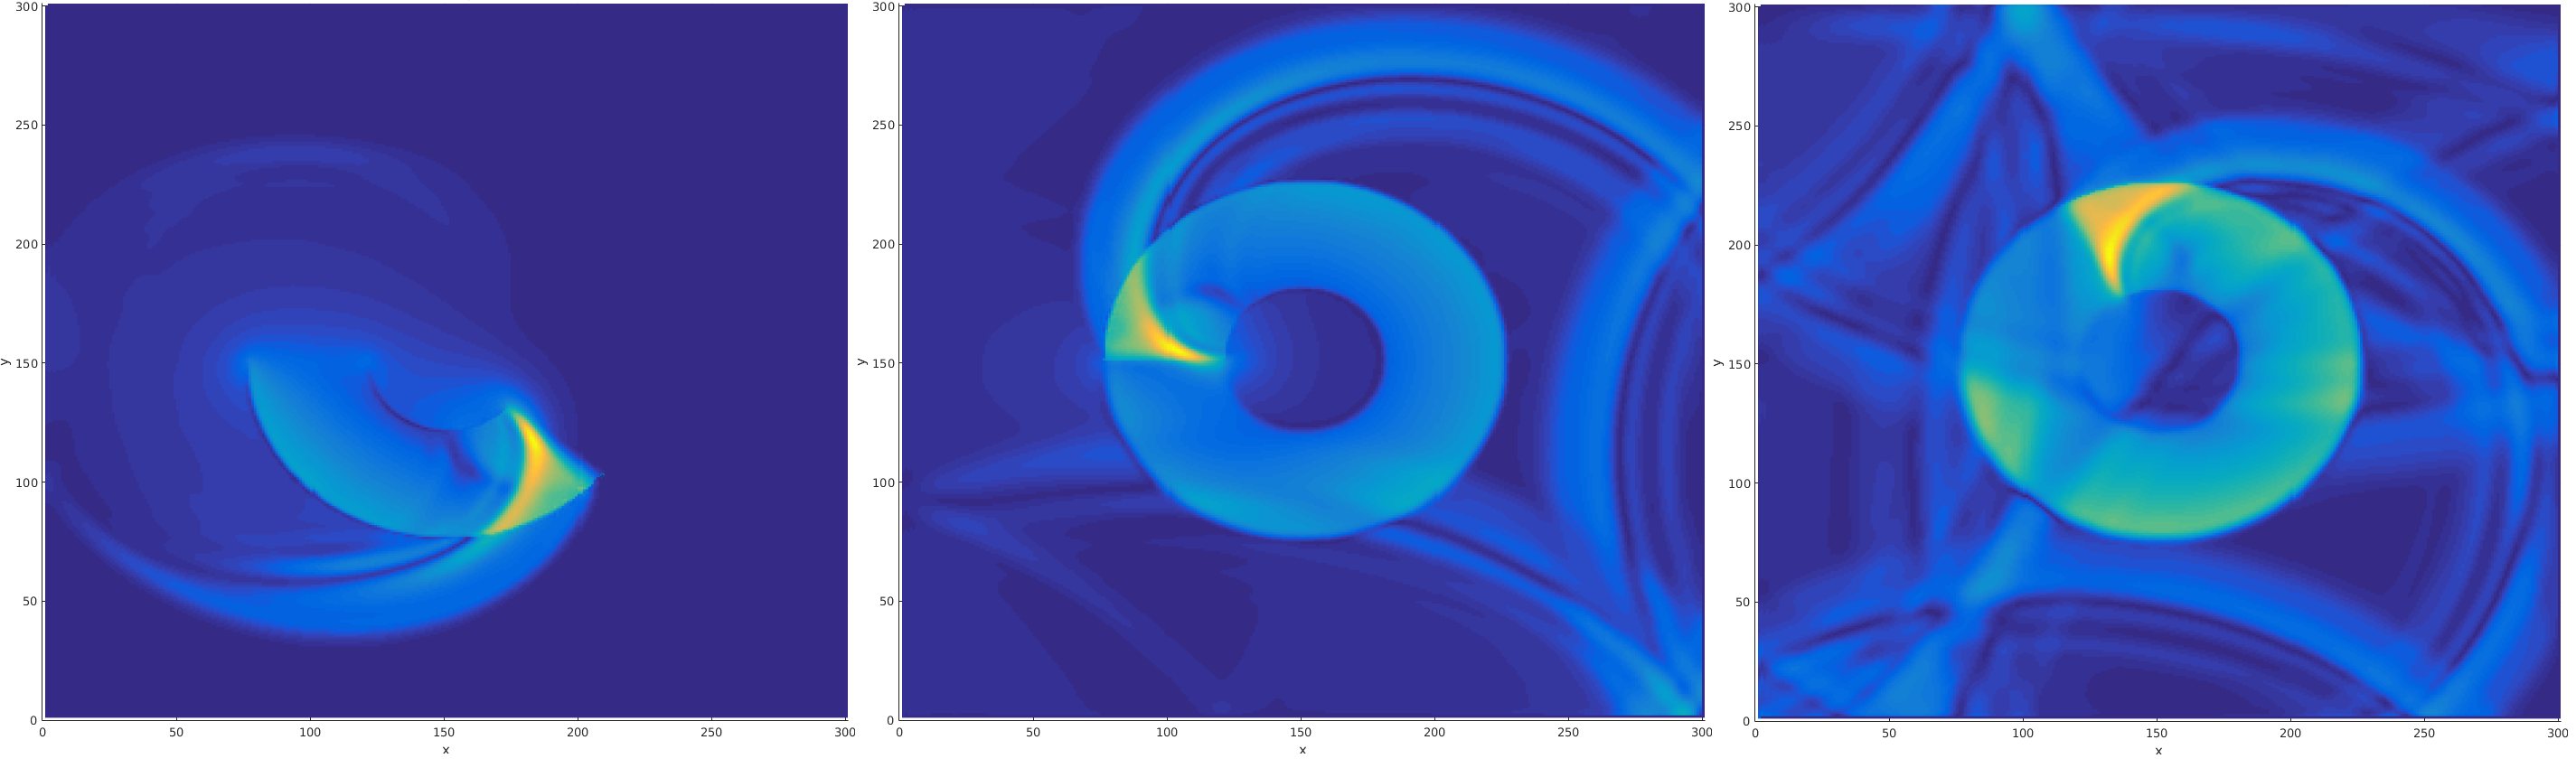
\includegraphics[width=\textwidth,height=4cm]{figures/sim_hm_all}
\caption{Estos mapas de calor muestran la evolución del fluido en el tiempo.}
\label{fig:sim_hm_all}
\end{figure*}

\begin{figure*}
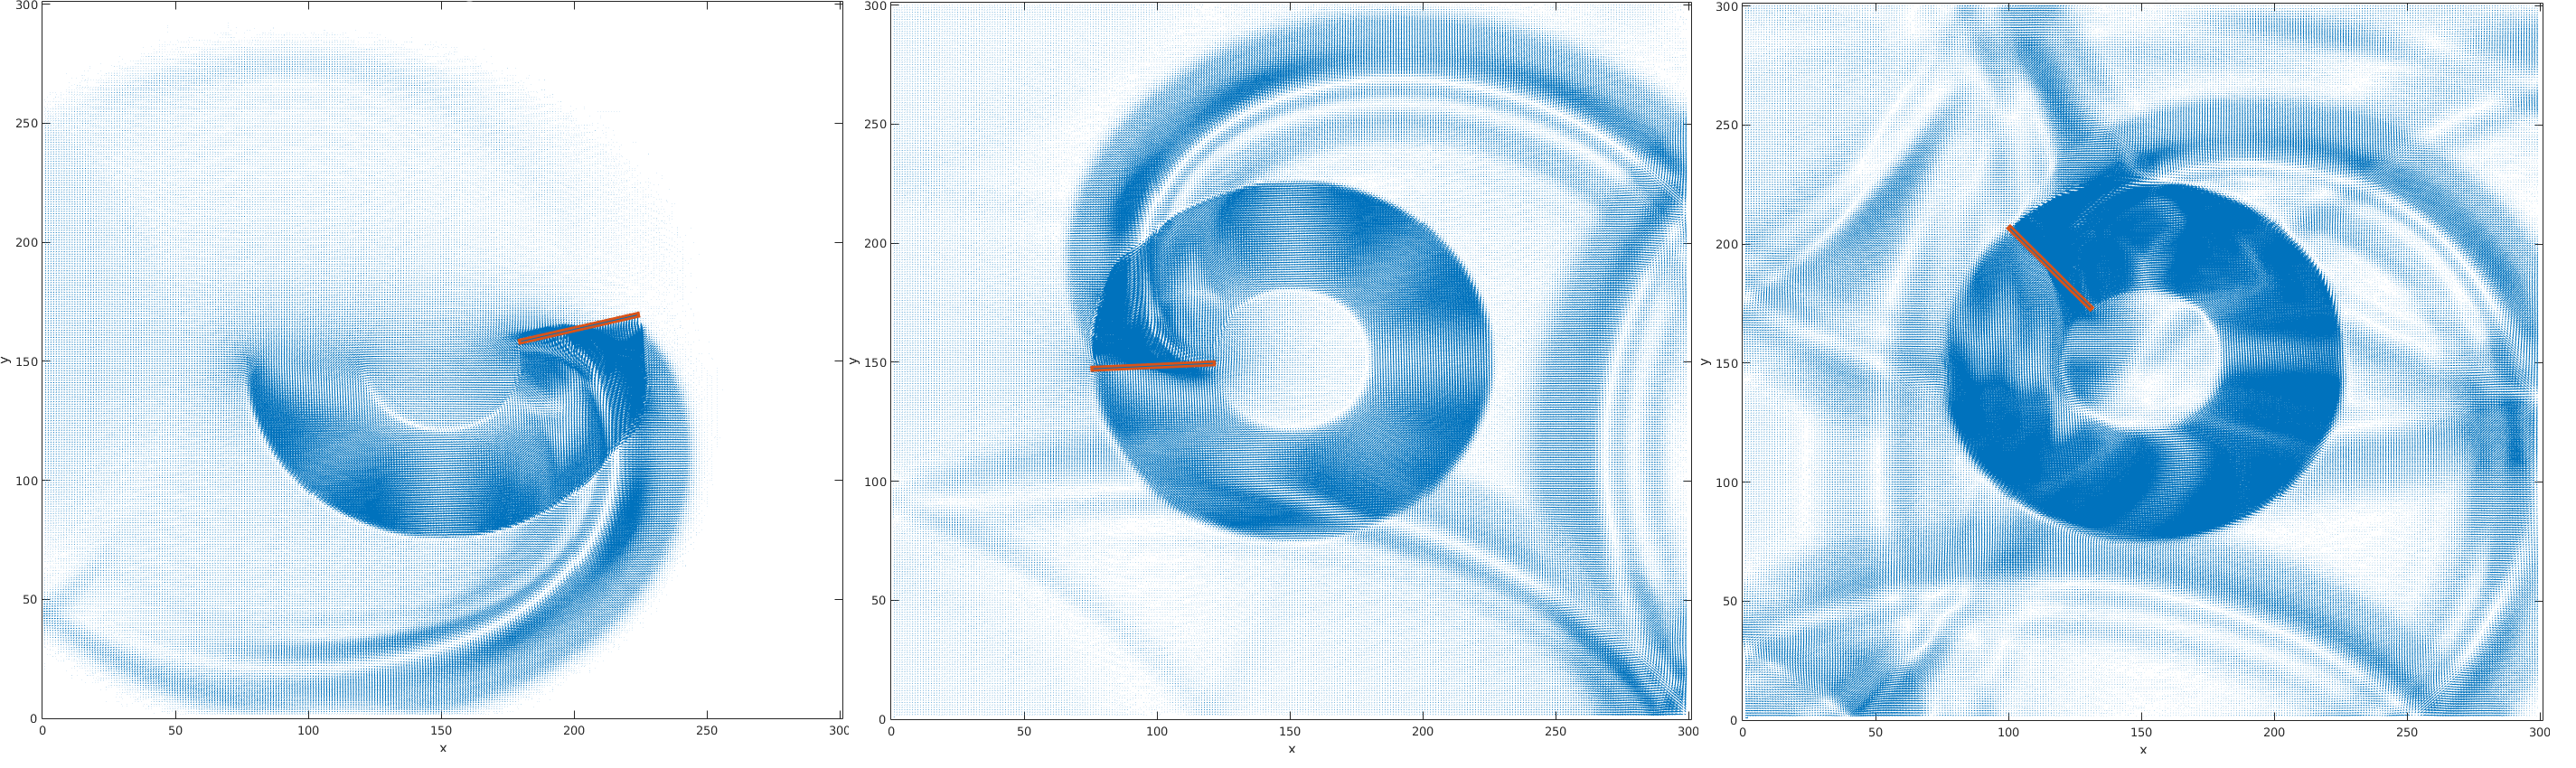
\includegraphics[width=\textwidth,height=4cm]{figures/sim_vf_all}
\caption{El aspa (rojo) empuja al fluido al rotar.}
\label{fig:sim_vf_all}
\end{figure*}

Como puede verse se aprecia claramente la posición del aspa rotante que empuja el fluido, asi como las ondas producidas por este movimiento. Tambien estas ondas reflejan correctamente en la pared del contenedor, y la dirección de rotación obtenida es la esperada por el empuje de un aspa moviendose en esa dirección.

~\\
Fueron realizados estudios de rendimiento, tratando de medir el impacto de la ejecución en paralelo. Como marco teórico de esta sección, se utilizó por un lado la Ley de Amdahl, midiendo así el speedup  $S(n,p) = \frac{T_{ser}(n) }{ T_{par}(n,p)}$  a trabajo fijo aumentando la cantidad de procesadores, y por otro la Ley de Gustavson para la cual medimos el trabajo realizado por cantidades cada vez mas grandes de recursos de procesamiento a tiempo constante, y luego calculamos la eficiencia $E(n,p) = \frac{S(n,p)}{p}$. Donde $ T_{ser}(n)$  es el tiempo que tarda el programa en su versión serial para una entrada de tamaño n, y $T_{par}(n,p)$  es el tiempo que tarda el programa paralelo para una entrada de tamaño n y cantidad de procesos p.

\begin{subsection}{Ley de Amdahl}
~\\
La Ley de Amdahl nos da el speedup teórico en la ejecución de una tarea que consta de una cantidad de trabajo fijo al incrementar los recursos del sistema.
~\\
~\\
Llevada al limite, sirve para calcular la mejora máxima posible para una tarea que consta de una parte paralelizable, y una parte serial que no puede ser efectivamente paralelizada.
~\\
La formulación matemática de la Ley de Amdahl es la siguiente:
~\\
~\\
$S(s) \leq  \frac{1}{(1-p)+\frac{p}{s}}$
~\\
~\\
Donde S es el speedup total, s el speedup de la parte del programa que se favorece por el paralelismo, y p es la proporción de tiempo que era ocupada por la parte del programa que tiene speedup alguno. Se asume que todo el tiempo que no corresponde a p, o sea 1-p, se mantiene igual. Un resultado directo de esta ley es que incluso utilizando infinitos recursos, no puede aumentarse el speedup mas que:
~\\

$S(s) \leq  \frac{1}{1-p}$
~\\

Para este experimento se quiere dejar fija la cantidad de trabajo total realizado, y medir como cambia la velocidad al agregar unidades de procesamiento. 
~\\
~\\
El programa fue ejecutado en una red ethernet con 21 maquinas, cada una disponiendo de 4 núcleos. Al momento de realizar la experimentación, estas maquinas estaban siendo utilizadas, a razón de dos nucleos por maquina, con lo cual se disponía de 42 núcleos para procesar la prueba. Los speedups resultado son los siguientes:
~\\
\begin{minipage}{\linewidth}
\begin{tcolorbox}[colback=blue!5!white,colframe=blue!75!black,title=Speedup]
\begin{verbatim}
#CPU S(n,p)

30   19.8541013255
25   19.2648777129
20   17.4229950177
15   15.4322650675
12   12.3897738475
10   10.5198631716
9    9.1780910351
8    8.434695922
6    6.0758387804
5    5.0493848725
3    2.5275473744
1    1

\end{verbatim}
\end{tcolorbox}
\end{minipage}
Los datos de esta tabla pueden ser apreciados en la figura \ref{fig:exp_amdahl_speedup}
\\

\begin{figure}
\textbf{Speedup}

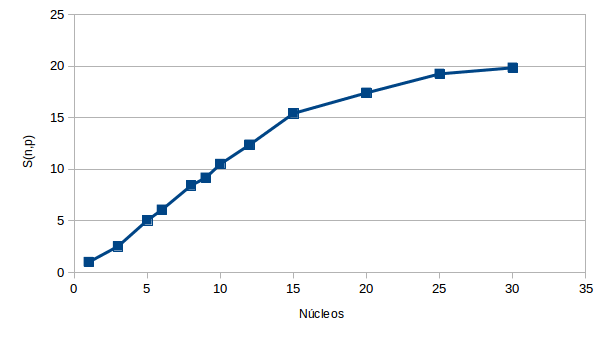
\includegraphics[width=\textwidth/2,height=\textheight/2,keepaspectratio]{figures/exp_amdahl_speedup}
\caption{El speedup tiende a disminuir al aumentar mucho la cantidad de nucleos, perdiendo approximadamente un tercio del rendimiento al alcanzar los 30.}
\label{fig:exp_amdahl_speedup}

\end{figure}

\end{subsection}


\begin{subsection}{Ley de Gustavson}
~\\
La Ley de Gustafson calcula el speedup teórico para una tarea de tiempo de ejecución fijo al incrementar los recursos de un sistema. Al aplicar la Ley de Gustavson, lo que varia no es el tiempo de ejecución, sino la cantidad de trabajo realizado. La formulación matemática de la Ley de Gustavson es la siguiente:
~\\
{\centering
$S(s) = p - \alpha(p-1)$
}
~\\
Donde S es el speedup, p es el número de procesadores, y $\alpha$ la parte no paralelizable del proceso. Notar que si se aumenta notablemente la el trabajo total en la sección paralelizable, haciendo que la proporción de trabajo serial $\alpha$ sea muy pequeña, esto resulta en algo muy similar a $S(s) = p$
~\\
Segun Guftavson, en su trabajo de 1988, tiene mucho mas sentido hablar de tiempo fijo que de tamaño fijo. Esto es así porque en la practica los timepos utilizados para realizar simulaciónes no varian tanto como los tamaños o cantidad de recursos utilizados para las mismas. Siguiendo este espiritu, en este experimento se quiere dejar el tiempo limite en 120s, y medir cuanta utilidad, o trabajo neto, pudo extraerse para distintas cantidades de unidades de procesamiento.
~\\
Para lograr esto, programa fue nuevamente ejecutado en una red ethernet con 21 maquinas, cada una disponiendo de 3 núcleos. Al momento de realizar la experimentación, estas maquinas estaban siendo utilizadas, a razón de un núcleo por maquina, con lo cual se disponía de 63 núcleos para procesar la prueba. 
~\\
~\\
Como medida de trabajo efectivo, se contó la cantidad de elementos del sistema calculados, ya que es lo que da utilidad. Se aclara que cuando en la tabla de resultados figura que se utilizó un solo núcleo, esa medición fue realizada sobre la versión serial del programa, no perdiendo así tiempo inicializaciónes o calculos necesarios para paralelizar. Los resultados son los siguientes, que tambien pueden apreciarse en la figura \ref{fig:exp_gustafson_work}. Tambien se calcula el trabajo normalizado por nucleo, obteniendose asi los datos que se ven en la figura \ref{fig:exp_gustafson_work_norm}
~\\
\begin{minipage}{\linewidth}

\begin{tcolorbox}[colback=blue!5!white,colframe=blue!75!black,title=Trabajo]
\begin{verbatim}
#CPU   elementos calculados
1      111.113 Millones
5      413.814 Millones
20     1976.24 Millones
35     3198.04 Millones
50     3661.31 Millones
60     4294.03 Millones
\end{verbatim}
\end{tcolorbox}
\end{minipage}

\begin{figure}
\textbf{Trabajo}

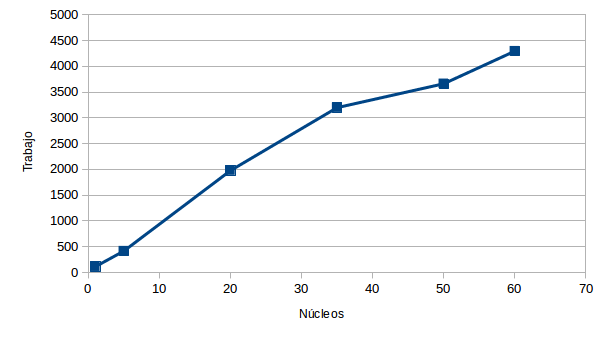
\includegraphics[width=\textwidth/2,height=\textheight/2,keepaspectratio]{figures/exp_gustafson_work}
\caption{el trabajo neto calculado se comporta de forma aproximadamente lineal.}
\label{fig:exp_gustafson_work}
\end{figure}
\begin{minipage}{\linewidth}
Los datos parecen indicar un comportamiento que escala correctamente con la cantidad de núcleos. En la siguiente tabla sin embargo, se muestra el trabajo por nucleo, y se ve que decrece con el aumento de los recursos.

\begin{tcolorbox}[colback=blue!5!white,colframe=blue!75!black,title=Trabajo por núcleo]
\begin{verbatim}
#CPU   trabajo/núcleos
1      111.113
5      82.7628
20     98.8120
35     91.3725
50     73.2262
60     71.5671
\end{verbatim}
\end{tcolorbox}
\end{minipage}

\begin{minipage}{\linewidth}

En particular, si normalizamos los datos respecto del trabajo realizado por la version serial, notamos una reducción del rendimiento de la simulación que llega a bajar hasta un 64\% respecto del rendimiento extraido por un solo núcleo.
\begin{tcolorbox}[colback=blue!5!white,colframe=blue!75!black,title=Trabajo normalizado]
\begin{verbatim}
#CPU  trabajo/(núcleos*111.113)
1     1
5     0.7448
20    0.8892
35    0.8223
50    0.6590
60    0.6440
\end{verbatim}
\end{tcolorbox}
\end{minipage}

\begin{figure}
\textbf{Trabajo normalizado}

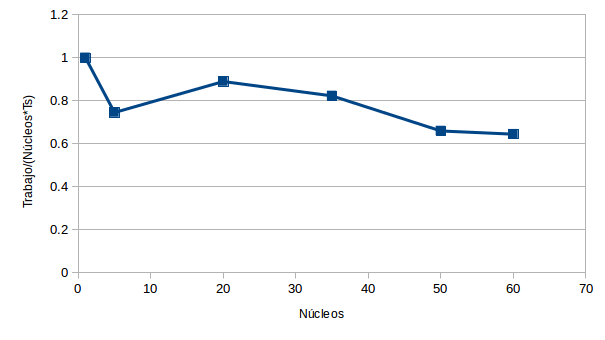
\includegraphics[width=\textwidth/2,height=\textheight/2,keepaspectratio]{figures/exp_gustafson_work_norm}
\caption{Al normalizar se nota mas facilmente la desviación de la linealidad.}
\label{fig:exp_gustafson_work_norm}

\end{figure}



~\\

 A primera vista, parece que se pierde mucho rendimiento. En realidad, si tenemos en cuenta que la corrida de un solo nucleo fue realizada con una versio distinta que no incluye codigo de MPI, se entiende que ese valor aparezca como un outlier. Dicho esto, lo que esperariamos ver si el programa escalara, seria una recta horizontal. Si bien no es el resultado obtenido, no se dista mucho. Lo importante es que encontramos que se puede aumentar la cantidad de trabajo realizable significativamente agregando unidades de procesamiento, lo cual es un resultado mas optimista que el insinuado por la Ley de Amdahl.
~\\
~\\
Otra medida importante relacionada con la ley de Gustafson, que ya fue mencionada anteriormente es la eficiencia. Con el objetivo de medir la eficiencia se realizó otra experimentación en la cual variara la cantidad de nucleos y el tamaño del problema, de forma tal de poder calcular el tiempo de ejecución y asi, la eficiencia. Recordemos que la definición de eficiencia es  $E(n,p) = \frac{S(n,p)}{p}$.
~\\
\begin{minipage}{\linewidth}
Los tiempos conseguidos en esta etapa de la experimentación son los siguientes.
~\\
\begin{tcolorbox}[colback=blue!5!white,colframe=blue!75!black,title=Tiempos]
\begin{verbatim}
#CPU raíz(2,n) Tp      Ts 

80   100       105.000 7731.128
40   75        74.730  2435.544
20   50        61.764s 713.772
5    50        252.129 713.772
1    1         0.366   0.366
\end{verbatim}
\end{tcolorbox}
\end{minipage}
Con lo cual la eficiencia en funcion de la cantidad de núcleos sería:
~\\
\begin{minipage}{\linewidth}
\begin{tcolorbox}[colback=blue!5!white,colframe=blue!75!black,title=Eficiencia]
\begin{verbatim}

#CPU eficiencia
80   0.920372381
40   0.8147812124
20   0.5778220323
5    0.5661958759
1    1
\end{verbatim}
\end{tcolorbox}
\end{minipage}

Si vemos la figura \ref{fig:exp_gustafson_eficiency}, encontramos devuelta que si bien la eficiencia no es optima, el resultado es mucho mejor que el esperado al seguir el paradigma planteado por la ley de Amdahl. Tambien puede verse nuevamente la diferencia entre la version serial y la version paralela para tareas de poco trabajo en el primer punto del grafico.
Como nota aparte, la eficiencia es una medida mucho mas sensible de la escalabilidad que el speedup, como podemos apreciar si comparamos este ultimo grafico, con el grafico de speedup (figura \ref{fig:exp_gustafson_speedup}) de los mismos datos.





\begin{figure}
\textbf{Eficiencia}
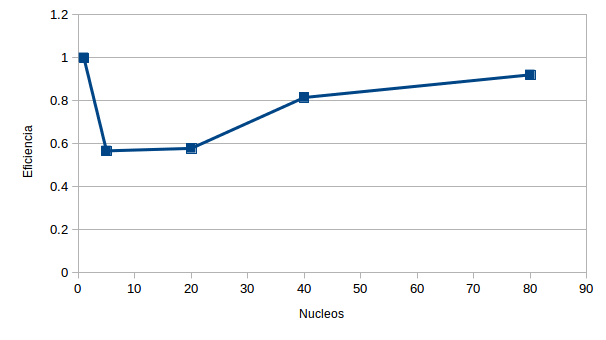
\includegraphics[width=\textwidth/2,height=\textheight/2,keepaspectratio]{figures/exp_gustafson_eficiency}
\caption{La eficiencia esta normalizada en función de la cantidad de núcleos, por lo que es muy sensible a las desviaciones de la linealidad.}
\label{fig:exp_gustafson_eficiency}
\end{figure}


\begin{figure}
\textbf{Speedup}
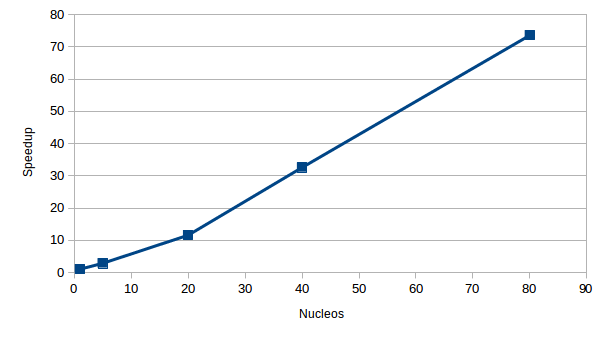
\includegraphics[width=\textwidth/2,height=\textheight/2,keepaspectratio]{figures/exp_gustafson_speedup}
\caption{Al graficar el speedup, se nota mucho menos el comportamiento no lineal.}
\label{fig:exp_gustafson_speedup}
\end{figure}

\end{subsection}
\end{section}
